\documentclass{standalone}
\begin{document}
	\subsection{Pipeline Structure}
	
	In this section I will discuss the general structure of the pipeline, more details about the actual implementation will be given in the next chapter.
	To perform the color quantization I've to found the characteristic color(centroids in the color space) of each tissue and use these colors for the actual segmentation, so the pipeline will be divided int two main steps. Before each of these steps we need a preliminary phase that aim to isolate the lung regions in order to exclude the extra lung areas and reduce the false positives.
	In the end the pipeline structure is divided in three main blocks as we can see in \figurename\,\ref{fig:Pipeline} : 
	\begin{itemize}
		\item \textbf{Pre-Processing and lung extraction}: Preliminary step, involves registration of HU, isolation of lung regions and reduction of motion artifacts;
		\item \textbf{Training} : estimation of the centroids, is performed only ones; 
		
		\item \textbf{Labeling} :  assignment of each voxel to the cluster of the closest centroids, it is the actual segmentation.
	\end{itemize}
	
		
	\begin{figure}[h!]
		\centering 
			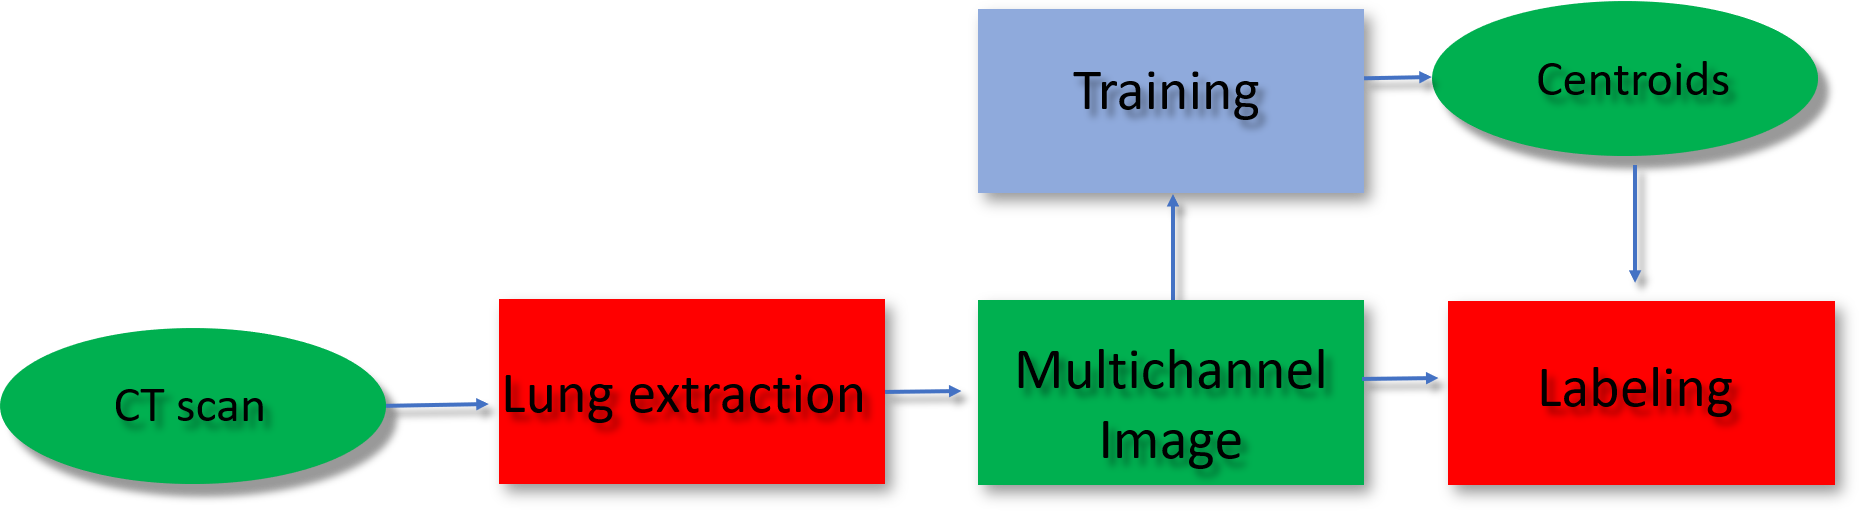
\includegraphics[width=.7\textwidth]{Pipeline.png}
		\label{fig:Pipeline}\caption{Flow chart of the main structure of the developed pipeline. The training process, which allows the estimation of the centroids, is performed only one time.}
	\end{figure} 
	
	\subsubsection*{Pre Processing and Lung Extraction}
	
	This preliminary step is performed before both training and labeling.\\
	First of all performs a registration of the HU on a common space, in order to overcomes the issues that may raise from the different padding values and multiplicative constant for HU computation(equation\,\ref{eq:HU}) used by the different manufacturer of the CT scans.\\
	This process is followed by a segmentation fo the lung regions, which allows to remove all the extra lung regions avoiding the formation of false positives. During this process a particular attention was paid on the removal of the main bronchial structures, which can interfere with the actual segmentation, and the preservation of the lung regions which are the ones in which we are interested in. An other aims of this step is the reduction of the motion artifacts caused by respiratory and cardiac cycle, which interferes with the actual segmentation since they may be wrongly classified as infection regions.
	
	\subsubsection*{Training}
	
	This step involves the estimation of the centroids for each tissue. To achieve this purpose we have chose to perform a clustering by using the kmeans algorithm. We have to takes into account that the kmenas clustering requires an homogeneous representation for each cluster. As we will see we have to manage this problem. One way to overcome this issue is to select several CT scans, which may be time consuming, or we can carefully select only one scan which provides an homogeneous representation of each cluster, as I've done in this work.\\
	In summary, the implementation of this step involve the building of the multi-channel image, which allow us to takes into account also the neighbouring information, the managing of the over represented clusters  and the actual centroids estimation.

	\subsection*{Labeling}
	
	This step involves the actual segmentation. The script which perform it requires as inputs the CT scans after the lung extraction, and the previously estimated centroids. This block of the pipeline simply assign each voxel to the cluster corresponding to the nearest centroids and the select only the one corresponding to GGO and CS. In this way we are performing a pixel classification by assign regions to a particular labels according only to intensities information, without exploiting spatial information: this allow us to group on the same cluster objects that are spatially disconnected as often happen in medical imaging field.\\
	The distance between voxel color and each centroid is defined as euclidean distance :
	\begin{equation*}
		d(x_j, c_i) = \sqrt{(x_j - c_i)^2}
	\end{equation*} 
	Where $x_j$ is the color vector for the $jth$ voxel and $c_i$ is the $ith$ centroid.\\
	
	To summarize, once the centroids are estimated, the segmentation pipeline will results in $2$ main steps : \textbf{lung extraction} and \textbf{labeling}, as shown in \figurename\,\ref{fig:FinalPipeline} in which we can observe the flowchart of each step with an image that shown the partial results.
	
	\begin{figure}
		\centering
			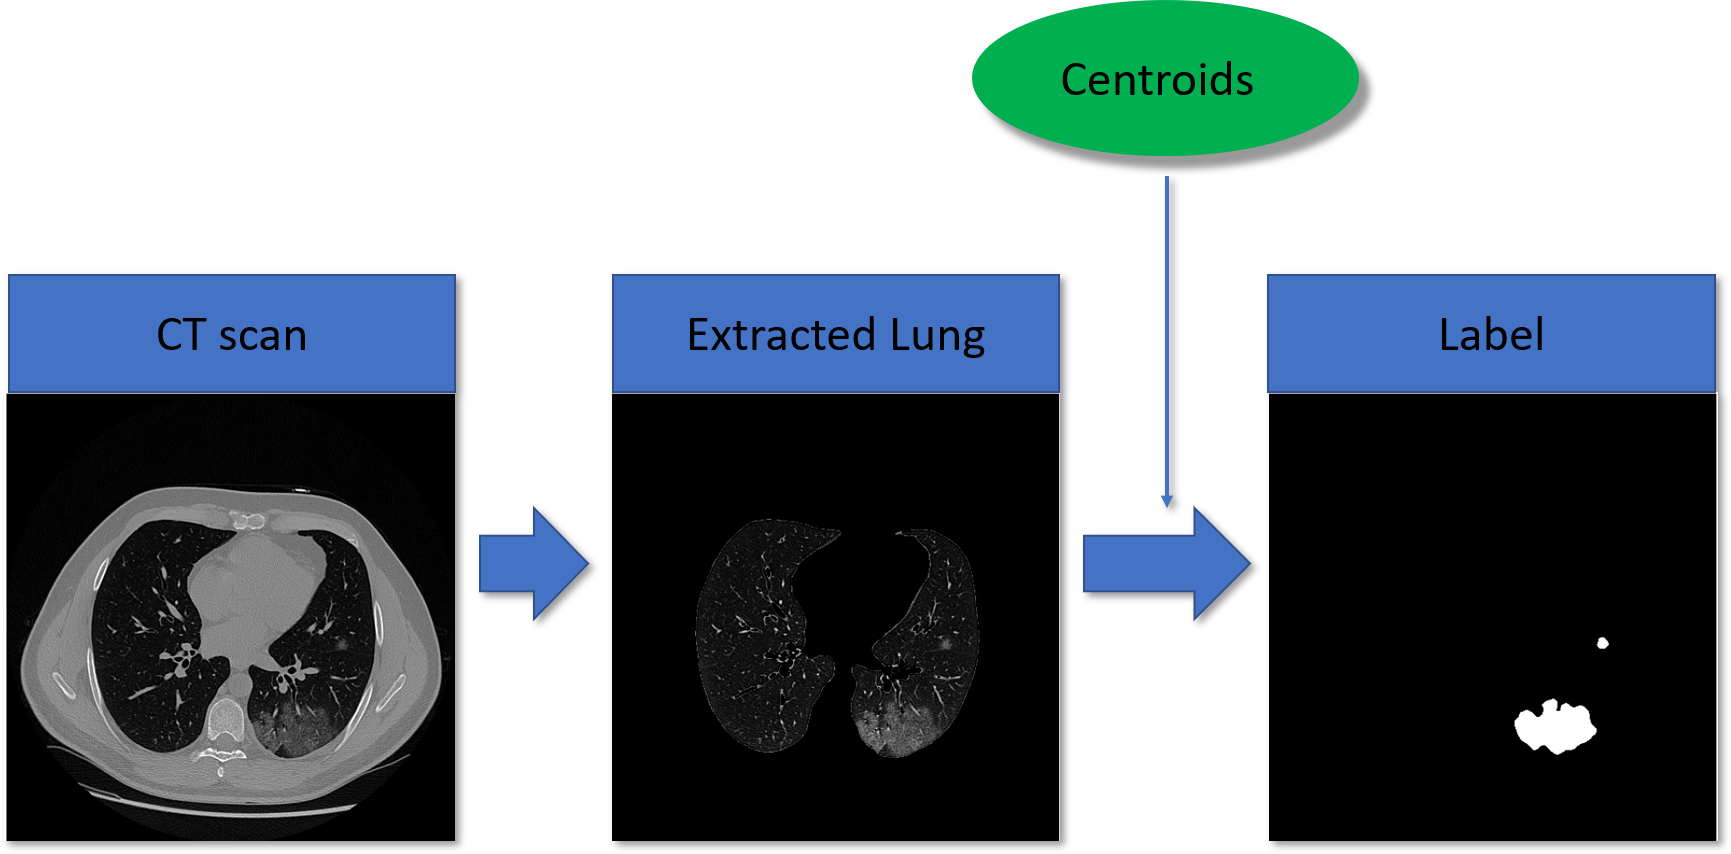
\includegraphics[width=.75\textwidth]{final_pipeline.png}
			\label{fig:FinalPipeline}\caption{Actual segmentation step, from left to right we can see the input image stack, the isolated lung regions and the final label. To performed the labeling a set of pre-computed centroids was used.}
	\end{figure}
	
	
	
\end{document}